\chapter{Assignment 3: Sets, Power Sets, Products, Families}\label{ch:sol3}

\subsection*{Problem 1}
This is Theorem~\ref{thm:empty}(c): $\varnothing\subseteq A$ for every set $A$, because the implication $x\in\varnothing\Rightarrow x\in A$ is vacuously true for every $x$ (there is no $x\in\varnothing$ to falsify it).

\subsection*{Problem 2}
Let $S_1=\{a_2X^2+a_1X+a_0:a_i\in\R\}$ (polynomials of degree $\le2$) and $S_2=\{a_4X^4+a_2X^2+a_0:a_i\in\R\}$ (polynomials with only even-degree terms, degree $\le4$). Both are non-empty subsets of $\R[X]$ (e.g.\ $0\in S_1\cap S_2$). Then:
\[
S_1\cap S_2=\{a_2X^2+a_0:a_2,a_0\in\R\}\qquad(\text{degree}\le2\text{ \emph{and} only even powers}),
\]
\[
S_1\cup S_2=\{a_2X^2+a_1X+a_0:a_i\in\R\}\cup\{a_4X^4+a_2X^2+a_0:a_i\in\R\}
\]
(polynomials that are either of degree $\le2$, or have only even-degree terms of degree $\le4$; e.g.\ $X^4\in S_1\cup S_2$ but $X^4\notin S_1\cap S_2$, and $X\in S_1\cup S_2$ but $X\notin S_1\cap S_2$).

\subsection*{Problem 3}
This is Theorem~\ref{thm:powersize}: if $\card(A)=n$ then $\card(\pset(A))=2^n$, proved by induction on $n$ by splitting $\pset(A)$ into the subsets that omit a fixed $a\in A$ (which biject with $\pset(A\setminus\{a\})$) and those that contain $a$ (which biject with the same set via $T\mapsto T\cup\{a\}$), giving $\card\pset(A)=2^n+2^n=2^{n+1}$ at the inductive step. See the full proof there.

\subsection*{Problem 4}
Recall from Chapter~\ref{ch:algebra} that a Venn diagram shades exactly those atoms whose truth-table row makes the given form true.

\begin{center}
	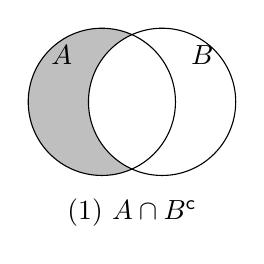
\begin{tikzpicture}[scale=0.85]
		\begin{scope}
			\clip (0,0) circle (1.1);
			\fill[gray!50] (-1.6,-1.6) rectangle (2.6,1.6);
		\end{scope}
		\begin{scope}
			\clip (0.9,0) circle (1.1);
			\fill[white] (-1.6,-1.6) rectangle (2.6,1.6);
		\end{scope}
		\draw (0,0) circle (1.1);
		\draw (0.9,0) circle (1.1);
		\node at (-0.6,0.7) {$A$};
		\node at (1.5,0.7) {$B$};
		\node[below] at (0.45,-1.3) {(1) $A\cap B^{\mathsf c}$};
	\end{tikzpicture}
	\hfill
	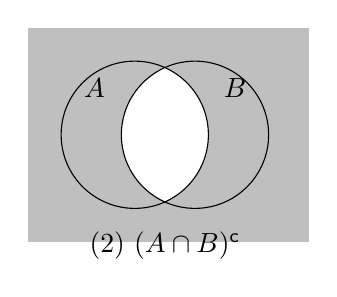
\begin{tikzpicture}[scale=0.85]
		\fill[gray!50] (-1.6,-1.6) rectangle (2.6,1.6);
		\begin{scope}
			\clip (0,0) circle (1.1);
			\clip (0.9,0) circle (1.1);
			\fill[white] (-1.6,-1.6) rectangle (2.6,1.6);
		\end{scope}
		\draw (0,0) circle (1.1);
		\draw (0.9,0) circle (1.1);
		\node at (-0.6,0.7) {$A$};
		\node at (1.5,0.7) {$B$};
		\node[below] at (0.45,-1.3) {(2) $(A\cap B)^{\mathsf c}$};
	\end{tikzpicture}
	\hfill
	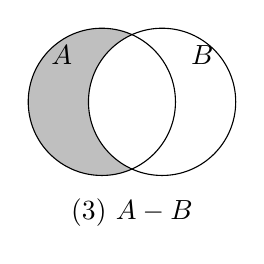
\begin{tikzpicture}[scale=0.85]
		\begin{scope}
			\clip (0,0) circle (1.1);
			\fill[gray!50] (-1.6,-1.6) rectangle (2.6,1.6);
		\end{scope}
		\begin{scope}
			\clip (0.9,0) circle (1.1);
			\fill[white] (-1.6,-1.6) rectangle (2.6,1.6);
		\end{scope}
		\draw (0,0) circle (1.1);
		\draw (0.9,0) circle (1.1);
		\node at (-0.6,0.7) {$A$};
		\node at (1.5,0.7) {$B$};
		\node[below] at (0.45,-1.3) {(3) $A-B$};
	\end{tikzpicture}
\end{center}
(Diagrams (1) and (3) come out identically shaded, which is exactly the content of $A\setminus B=A\cap B^{\mathsf c}$, Theorem~\ref{thm:setlaws}.)

As a check (and because a diagram alone is not a proof, Chapter~\ref{ch:algebra}), each shaded region is exactly the atom(s) predicted by the truth table:
\begin{center}
	\begin{tabular}{@{}p{3.6cm}p{3.6cm}p{6.4cm}@{}}
		\toprule
		\textbf{Set} & \textbf{Atoms shaded} & \textbf{Description}\\
		\midrule
		(1) $A\cap B\comp$ & $(\T,\F)$ & the crescent of $A$ outside $B$ — same as $A\setminus B$\\
		(2) $(A\cap B)\comp$ & $(\T,\F),(\F,\T),(\F,\F)$ & everything except the lens $A\cap B$\\
		(3) $A-B$ & $(\T,\F)$ & identical shading to (1), confirming $A\setminus B=A\cap B\comp$ (Theorem~\ref{thm:setlaws})\\
		\bottomrule
	\end{tabular}
\end{center}
(Here $(\T,\F)$ denotes the atom ``in $A$, not in $B$'', etc., as in the table of Chapter~\ref{ch:algebra}.) That (1) and (3) shade the same atom is exactly the identity $A\setminus B=A\cap B\comp$.

\subsection*{Problem 5}
This is Theorem~\ref{thm:setlaws}, proved by the direct method (via the logic--set dictionary): for $x\in X$,
\[
x\in(A\cap B)\comp\iff\neg(x\in A\wedge x\in B)\iff x\notin A\vee x\notin B\iff x\in A\comp\cup B\comp,
\]
\[
x\in(A\cup B)\comp\iff\neg(x\in A\vee x\in B)\iff x\notin A\wedge x\notin B\iff x\in A\comp\cap B\comp,
\]
using De Morgan's laws of propositional logic (Theorem~\ref{thm:laws}) at the middle step, and Extensionality to conclude set equality. See the full proof in Chapter~\ref{ch:algebra}.

\subsection*{Problem 6}
(a) This is Theorem~\ref{thm:product-laws}(a): if $T\subseteq A$ then for $(t,b)\in T\times B$, $t\in T\subseteq A$ and $b\in B$, so $(t,b)\in A\times B$.

(b) This is Theorem~\ref{thm:product-laws}(b): $(a,b)\in A\times(B\cup C)\iff a\in A\wedge(b\in B\vee b\in C)\iff(a\in A\wedge b\in B)\vee(a\in A\wedge b\in C)\iff(a,b)\in(A\times B)\cup(A\times C)$.

\subsection*{Problem 7}
$A_n=[-\tfrac1n,\tfrac1n]$, $n\ge1$. Since $1/n$ is decreasing, $A_1\supseteq A_2\supseteq A_3\supseteq\cdots$ (each $A_{n+1}\subseteq A_n$ as $\frac1{n+1}<\frac1n$). Hence:
\[
\bigcup_{n=1}^\infty A_n=A_1=[-1,1]\qquad(\text{the largest set in a decreasing chain is the first}).
\]
\[
\bigcap_{n=1}^\infty A_n=\{0\}.
\]
Indeed $0\in A_n$ for every $n$; and if $x\ne0$, the Archimedean property gives $n>1/|x|$, so $|x|>1/n$ and $x\notin A_n$, whence $x\notin\bigcap_nA_n$.
\[
\prod_{n=1}^\infty A_n=\Bigl\{(x_n)_{n\ge1}:x_n\in\Bigl[-\tfrac1n,\tfrac1n\Bigr]\text{ for every }n\Bigr\}\subseteq\R^{\N_{\ge1}}:
\]
this is a \emph{set of sequences} (Chapter~\ref{ch:functions}, Definition~\ref{def:product}), not a subset of $\R$; it is quite different in kind from the union and intersection above.

\subsection*{Problem 8}
$A_n=\{1,\dots,n\}$, $n\ge1$. Then
\[
\prod_{n=1}^\infty A_n=\Bigl\{f:\N_{\ge1}\to\textstyle\bigcup_nA_n\ :\ f(n)\in\{1,\dots,n\}\text{ for every }n\Bigr\},
\]
i.e.\ the set of all sequences $(x_n)_{n\ge1}$ with $x_n\in\{1,\dots,n\}$ — so $x_1=1$ necessarily, $x_2\in\{1,2\}$, $x_3\in\{1,2,3\}$, and so on, with more freedom at later indices.

\emph{Two elements:} $(x_n)=(1,1,1,1,\dots)$ (constantly $1$; valid since $1\in\{1,\dots,n\}$ for every $n$), and $(x_n)=(1,2,3,4,\dots)$, i.e.\ $x_n=n$ (valid since $n\in\{1,\dots,n\}$).

\emph{A sequence not in the product:} $(x_n)=(1,3,3,3,\dots)$, i.e.\ $x_2=3\notin\{1,2\}=A_2$; this fails already at $n=2$.

\subsection*{Problem 9}
$A_n=(-n,1-\tfrac1n)$, $n\ge1$ (for $n=1$, $A_1=(-1,0)$). As $n$ increases, the left endpoint $-n\to-\infty$ and the right endpoint $1-\frac1n$ increases toward (but never reaches) $1$; one checks $A_n\subseteq A_{n+1}$ (since $-n>-(n+1)$ and $1-\frac1n<1-\frac1{n+1}$), so the family is increasing.
\begin{claim}
	$\bigcup_{n=1}^\infty A_n=(-\infty,1)$.
\end{claim}
\begin{proof}
	($\subseteq$) Every $A_n\subseteq(-\infty,1)$ since $1-\frac1n<1$. ($\supseteq$) Let $x<1$. By the Archimedean property choose $n$ with $n>-x$ (so $x>-n$) and, using density/Archimedean again, $n$ large enough that $1-\frac1n>x$ (possible since $1-\frac1n\to1>x$); taking the larger of the two required $n$'s gives $x\in A_n$.
\end{proof}

\subsection*{Problem 10}
$H_n=\{(x,y)\in\R^2:y\ge-n\}$, $n\ge1$. The family is increasing: if $y\ge-n$ then, since $-n>-(n+1)$, we get $y\ge-n>-(n+1)$, so $y\ge-(n+1)$ too; hence $H_n\subseteq H_{n+1}$.

\emph{Union.} $\bigcup_{n\ge1}H_n=\R^2$. Given any $(x,y)\in\R^2$, the Archimedean property provides $n\in\N$ with $n>-y$, i.e.\ $y>-n$, so $(x,y)\in H_n$.

\emph{Intersection.} $\bigcap_{n\ge1}H_n=H_1=\{(x,y):y\ge-1\}$. If $(x,y)\in\bigcap_nH_n$ then in particular $y\ge-1$ (the $n=1$ case). Conversely, if $y\ge-1$ then, as $H_n$ is increasing with smallest member $H_1$, $(x,y)\in H_1\subseteq H_n$ for every $n\ge1$.

\subsection*{Problem 11}
For the finite product $\R^r=\prod_{n=1}^rR$, the standard basis $\{e_1,\dots,e_r\}$ (with $e_i$ the tuple with a $1$ in position $i$, $0$ elsewhere) is a basis: it is independent (a vanishing combination $\sum a_ie_i=0$ forces each $a_i=0$ by comparing coordinates) and spans (any $(x_1,\dots,x_r)=\sum x_ie_i$, a genuine \emph{finite} sum since $r$ is finite).

For the infinite product $\prod_{n=1}^\infty\R$ (sequences $(x_n)_{n\ge1}$), \textbf{$\{e_1,e_2,\dots\}$ is NOT a basis.} It is still linearly independent (the same coordinate argument, applied to any finite sub-collection, Lemma~\ref{lem:span}-style reasoning). But it does not span: by Lemma~\ref{lem:span}, $\Span\{e_1,e_2,\dots\}$ consists only of \emph{finite} linear combinations $a_1e_{n_1}+\dots+a_ke_{n_k}$, which are exactly the sequences with only \emph{finitely many} non-zero terms. The sequence $(1,1,1,\dots)$ (constantly $1$) has infinitely many non-zero terms, so it is \emph{not} in $\Span\{e_1,e_2,\dots\}$; hence $\{e_1,e_2,\dots\}$ does not span $\prod_{n=1}^\infty\R$ and is not a basis. (A basis of $\prod_{n=1}^\infty\R$ does exist, by Theorem~\ref{thm:basis}, but — being infinite-dimensional — it cannot be exhibited explicitly; this is a genuinely non-constructive use of Zorn's Lemma / the Axiom of Choice, Chapter~\ref{ch:zorn}.)

\subsection*{Problem 12}
Suppose $A_{j_0}=\varnothing$ for some fixed $j_0\in\N$, within the family $\{A_n\}_{n\in\N}$.
\begin{itemize}
	\item $\bigcup_{n\in\N}A_n$: nothing forced in general. The empty set contributes nothing to a union ($A_{j_0}$ drops out, Proposition~\ref{prop:binunion}), but the union of the \emph{other} $A_n$'s can be anything, including all of some ambient set; no general conclusion follows purely from $A_{j_0}=\varnothing$.
	\item $\bigcap_{n\in\N}A_n=\varnothing$ \textbf{necessarily.} Since $\bigcap_nA_n\subseteq A_{j_0}=\varnothing$ (an intersection is a subset of every one of its members, Definition~\ref{def:bigcap}), we get $\bigcap_nA_n=\varnothing$.
	\item $\prod_{n\in\N}A_n=\varnothing$ \textbf{necessarily}, by Theorem~\ref{thm:prodempty}(a): an element of the product would need a value $f(j_0)\in A_{j_0}=\varnothing$, impossible.
\end{itemize}